\chapter{Conclusion}

\section{Making an IDE is hard}

\begin{figure}
  \centering
  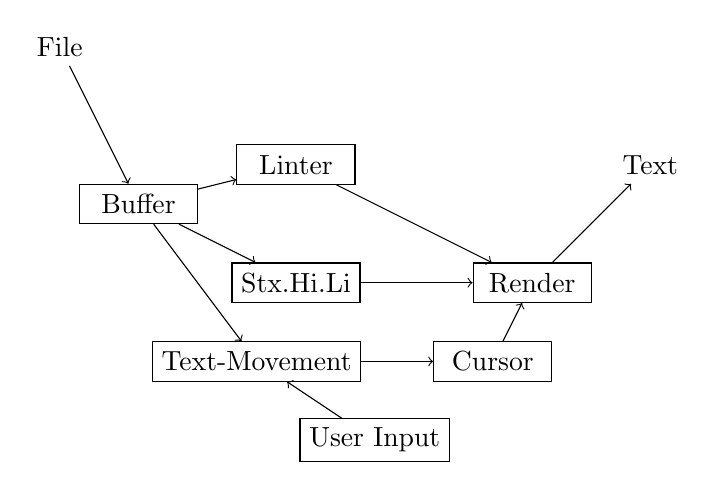
\begin{tikzpicture}
  % Nodes
  \node (file) [] at (-6, 3) {File};
  \node (parser) [rectangle, draw, minimum height=0.5cm, minimum width=1.5cm] at (-5, 1) {Buffer};
  \node (stxhili) [rectangle, draw, minimum height=0.5cm, minimum width=1.5cm] at (-3, 0) {Stx.Hi.Li};
  \node (text-movement) [rectangle, draw, minimum height=0.5cm, minimum width=1.5cm] at (-3.5, -1) {Text-Movement};
  \node (linter) [rectangle, draw, minimum height=0.5cm, minimum width=1.5cm] at (-3, 1.5) {Linter};
  \node (cursor) [rectangle, draw, minimum height=0.5cm, minimum width=1.5cm] at (-0.5, -1) {Cursor};
  \node (user-input) [rectangle, draw, minimum height=0.5cm, minimum width=1.5cm] at (-2, -2) {User Input};
  \node (render) [rectangle, draw, minimum height=0.5cm, minimum width=1.5cm] at (0, 0) {Render};
  \node (text) at (1.5, 1.5) {Text};
  % Arrow
  \draw[->] (file) -- (parser) node[midway, above] {};
  \draw[->] (parser) -- (stxhili) node[midway, above] {};
  \draw[->] (parser) -- (linter) node[midway, above] {};
  \draw[->] (parser) -- (text-movement) node[midway, above] {};
  \draw[<-] (render) -- (stxhili) node[midway, above] {};
  \draw[<-] (render) -- (linter) node[midway, above] {};
  \draw[<-] (cursor) -- (text-movement) node[midway, above] {};
  \draw[<-] (text-movement) -- (user-input) node[midway, above] {};
  \draw[->] (cursor) -- (render) node[midway, above] {};
  \draw[->] (render) -- (text) node[midway, above] {};
\end{tikzpicture}


  \caption{Text Editor Module Family}
  \label{fig:extendedModuleFamily}
\end{figure}

In the figure \ref{fig:extendedModuleFamily}, the \textit{cursor} is the place
at which text is placed when the user writes. If the user clicks someplace in
the document, the cursor \textit{jumps} to that place. If the user uses the
arrow-keys to move around, the cursor moves one character to left or right, or
one line up and down, depending on which arrow-key was pressed.
